%!TEX root = ../rapport.tex
%!TEX encoding = UTF-8 Unicode

% Chapitres "Introduction"

% modifié par Francis Valois, Université Laval
% 31/01/2011 - version 1.0 - Création du document


\label{s:experimentation}
\chapter{Rapport}
\label{cha:projet}
Ce laboratoire vise à concevoir une boucle de régulation dans le domaine discret et à valider la réalisation par une expérimentation pratique au laboratoire.
\section{Préparation}
Le procédé à analyser est présenté à l'équation suivante:
\begin{equation}
	G_p(s) = \frac{1}{(22s +1)(5s+1)}
\end{equation}
Il est nécessaire d'y inclure la présence du bloqueur d'ordre 0:
\begin{equation}
	G_{BOZ}(s) = \frac{1 - \mbox{e}^{-Ts}}{s}
\end{equation}
La période d'échantillonnage (T) est égale à 4 secondes. Le développement nécessaire à la détermination de la transformée en z est le suivant:
\begin{gather}
\overline{G_{BOZ}G_p}(z) = \mathcal{Z}\left\lbrace G_{BOZ}\right\rbrace \cdot \mathcal{Z}\left\lbrace G_{p}\right\rbrace\\
\overline{G_{BOZ}G_p}(z) = \mathcal{Z}\left\lbrace \frac{1 - \mbox{e}^{Ts}}{s}\right\rbrace \cdot \mathcal{Z}\left\lbrace \frac{\frac{1}{5 \cdot 22}}{(s + 1/22)(s+1/5)}\right\rbrace\\
\overline{G_{BOZ}G_p}(z) =  \left(\frac{z-1}{z}\right) \mathcal{Z}\left\lbrace \frac{\frac{1}{5 \cdot 22}}{s(s + 1/22)(s+1/5)}\right\rbrace\\
\overline{G_{BOZ}G_p}(z) =  \left(\frac{z-1}{z}\right) \mathcal{Z}\left\lbrace \frac{0.05882}{s(s + \frac{1}{22})} - \frac{0.05882}{s(s + \frac{1}{5})}\right\rbrace\\
\overline{G_{BOZ}G_p}(z) = \frac{-0.05882\cdot 5 (1-\mbox{e}^{\frac{-4}{5}})}{(z-\mbox{e}^{\frac{-4}{5}})} + \frac{0.05882\cdot 22(1-\mbox{e}^{\frac{-22}{5}})}{(z-\mbox{e}^{\frac{-22}{5}})}\\
\overline{G_{BOZ}G_p}(z) = \frac{0.05318z + 0.03837}{(z-0.4493)(z-0.8338)}
\end{gather}
On exprime $H(z)$ comme une fonction de z positifs. Il est possible de déterminer la fonction $H(z)$ à partir des données présentées dans le problème.
\begin{gather}
y(k) = 0.2r(k-1) + 0.4 r(k-2) + 0.3r(k-3) + 0.1r(k-4)\\
\frac{Y(z)}{R(z)} = 0.2z^{-1} + 0.4z^{-2} + 0.3z^{-3} + 0.1z^{-4}\\
H(z) = \frac{Y(z)}{R(z)} = \frac{0.2z^{3} + 0.4z^{2} + 0.3z^{1} + 0.1}{z^4}
\end{gather}
On vérifie que H(z=1) est bel et bien à gain unitaire.
Connaissant $\overline{G_{BOZ}G_p}(z)$ et $H(z)$, il est possible de déterminer le régulateur $G_c(z)$ nécessaire selon l'équation présentée ci-dessous:
\begin{gather}
G_c(z) = \frac{N_H(z)}{(D_H(z) - N_H(z)}\cdot \frac{1}{\overline{G_{BOZ}G_p}(z)}
\end{gather}
Il est possible de déterminer le régulateur à partir des paramètres déterminés précédemment:
\begin{gather}
G_c(z) = \frac{0.2z^{3} + 0.4z^{2} + 0.3z^{1} + 0.1}{z^4 - 0.2z^{3} - 0.4z^{2} - 0.3z^{1} - 0.1}\cdot \frac{(z-0.4493)(z-0.8338)}{0.05318z + 0.03837}
\end{gather}
On vérifie au moyen de la figure \ref{fig1} que le régulateur a exactement la réponse de la fonction de transfert désirée lorsqu'on applique un échelon de consigne unitaire.

\begin{figure}
\centering
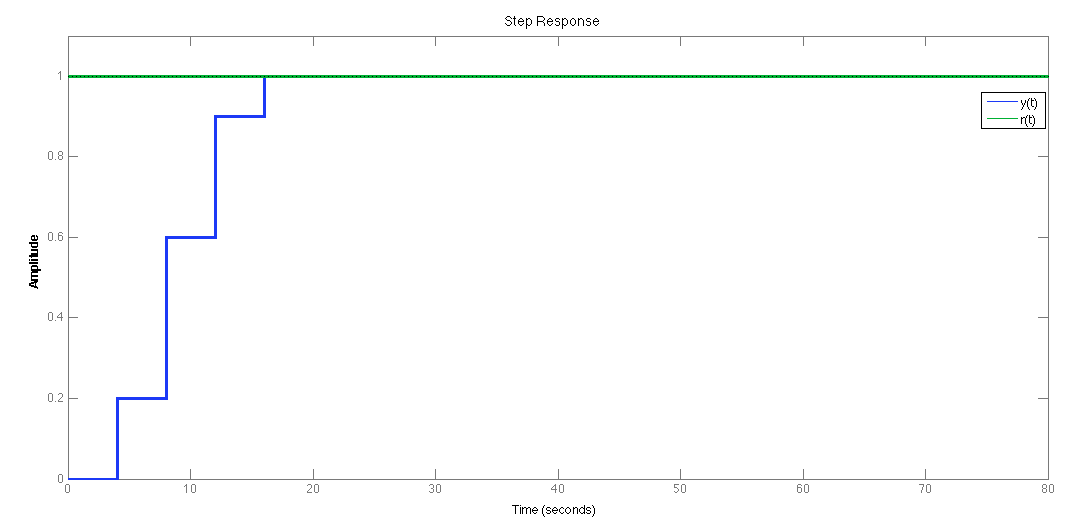
\includegraphics[scale=0.4]{fig_prep.png}
\caption{Réponse du système $G_p(s)$ pour un échelon de consigne unitaire lorsque régulé au moyen de $G_c(z)$}
\label{fig1}
\end{figure}
\section{Expérimentation}
Afin de corriger les paramètres théoriques du régulateur déterminé lors de la préparation, il est nécessaire de procéder à un essai d'identification du procédé analogique. La figure \ref{fig5} présente la réponse obtenue à un échelon unitaire de de consigne. Au moyen de ident, le procédé continu a été identifié comme le procédé suivant:
\begin{gather}
G_p(s) = \frac{1.0182}{(14.2776s +1)(3.2146s + 1)}
\end{gather}

Selon ident, le procédé identifié possède une corrélation de 99.67\% avec le modèle.

\begin{figure}[htbp]
\centering
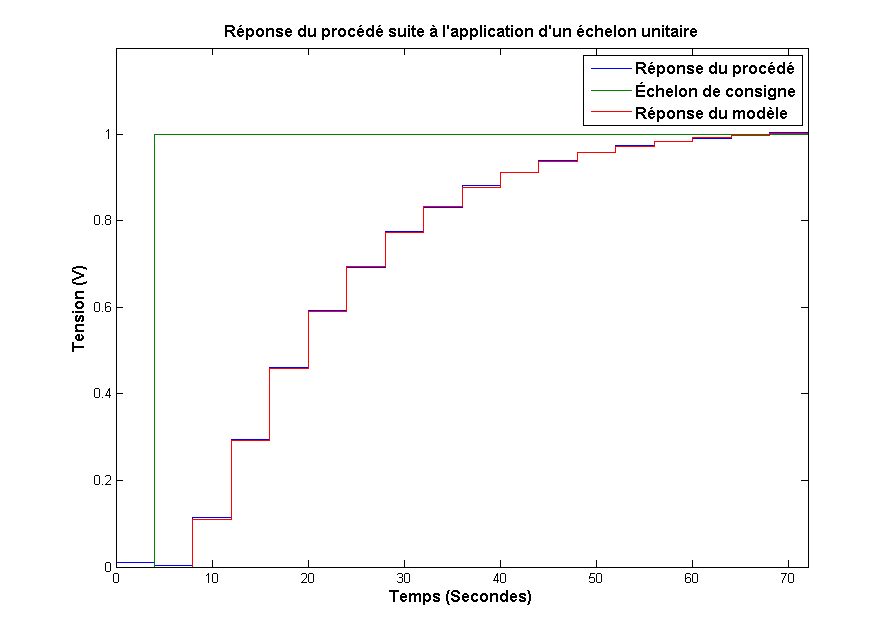
\includegraphics[scale=0.6]{procede_test.png}
\caption{Comparaison de la réponse à un échelon unitaire du procédé analogique discrétisé avec un temps d'échantillonnage de 4 secondes et du modèle déterminé au moyen de ident }
\label{fig5}
\end{figure}

Le temps d'échantillonnage étant de 4 secondes, il est possible d'effectuer la conversion vers le domaine discret directement dans matlab. Le procédé numérique résultant est présenté ci-dessous:
\begin{gather}
G_p(z) = \frac{0.1105z + 0.06664}{z^2 -1.044z + 0.2177}
\end{gather}
Comme le procédé est différent ce celui déterminé lors de la préparation, il est nécessaire de recalculer le régulateur numérique. Il est possible d'employer exactement le même développement que précédemment:
\begin{gather}
G_c(z) = \frac{0.2z^{3} + 0.4z^{2} + 0.3z^{1} + 0.1}{z^4 - 0.2z^{3} - 0.4z^{2} - 0.3z^{1} - 0.1}\cdot \frac{z^2 -1.044z + 0.2177}{0.1105z + 0.06664}
\end{gather}
Le schéma bloc du système d'asservissement numérique est présenté à la figure \ref{fig2} et a été réalisé de manière pratique dans le laboratoire. Afin de valider les performances, nous avons procédé à deux essais de validation, soit un essai avec un échelon unitaire et un essai avec un échelon de quatre. Les comparaisons entre les performances obtenues avec le modèle théorique et le prototype expérimental sont présentées aux figures \ref{fig3} et \ref{fig4} pour les essais avec un échelon unitaire et un échelon de quatre respectivement. 



\begin{figure}[htbp]
\centering
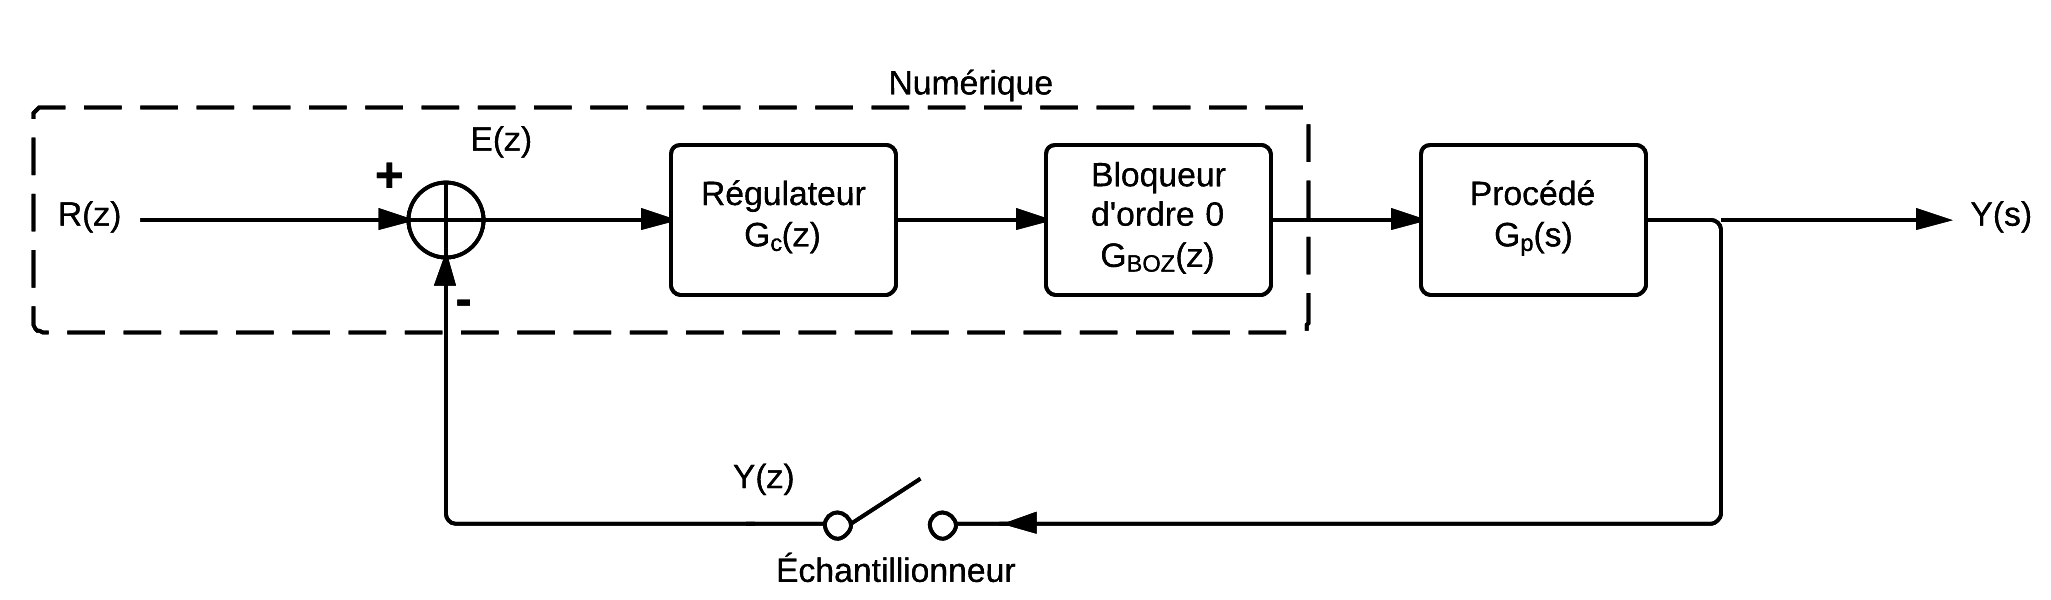
\includegraphics[scale=0.2]{lab6_commande.png}
\caption{Schéma bloc du système d'asservissement numérique du procédé analogique}
\label{fig2}
\end{figure}

\begin{figure}[htbp]
\centering
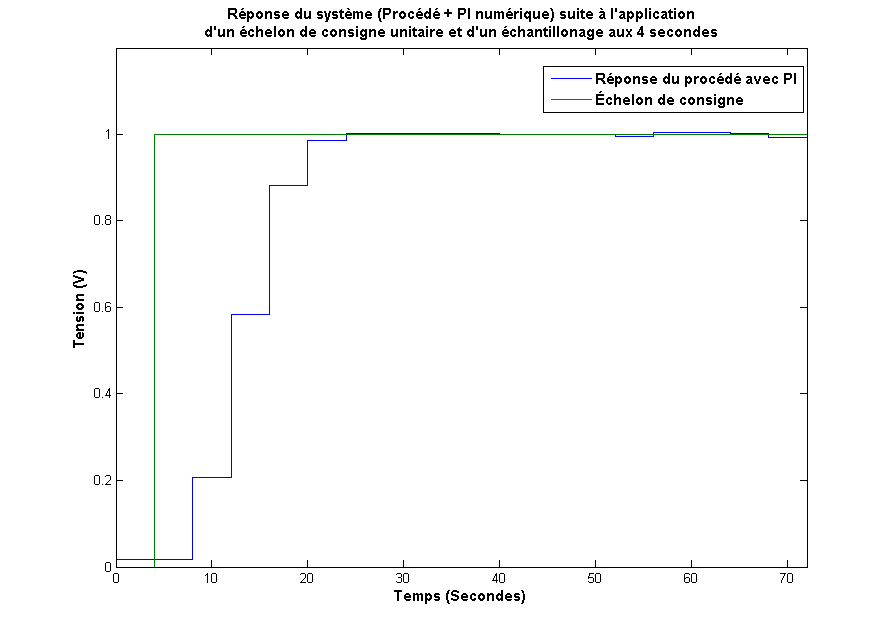
\includegraphics[scale=0.5]{essai1.png}
\caption{Résultats de l'essai de validation des performances au moyen d'un échelon unitaire sur le procédé analogique discrétisé avec un temps d'échantillonnage de 4 secondes.}
\label{fig3}
\end{figure}

\begin{figure}[htbp]
\centering
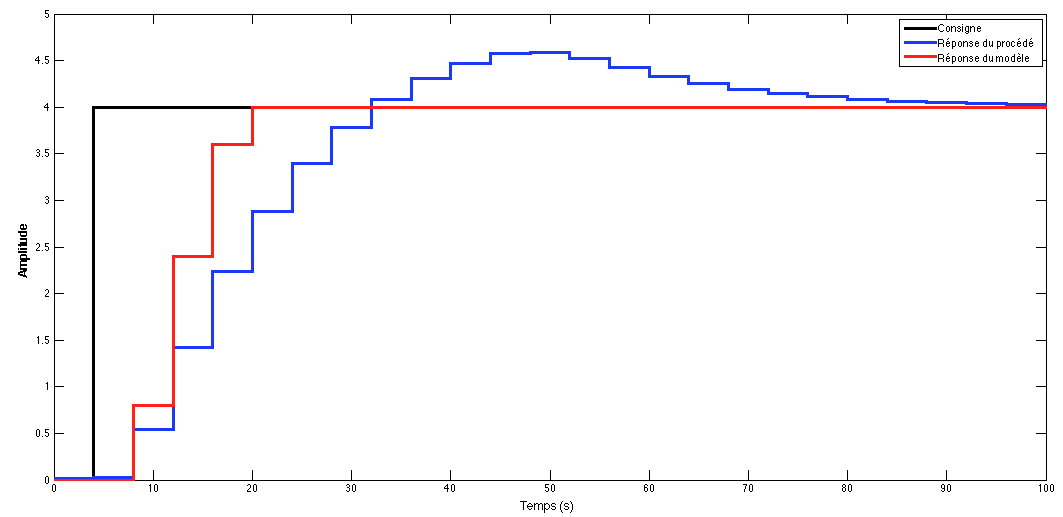
\includegraphics[scale=0.5]{essai2.png}
\caption{Résultats de l'essai de validation des performances au moyen d'un échelon de 4 sur le procédé analogique discrétisé avec un temps d'échantillonnage de 4 secondes.}
\label{fig4}
\end{figure}
\clearpage
\section{Discussion des résultats}
Au moyen de l'essai d'identification du modèle présenté à la figure \ref{fig5} il est possible de constater que la corrélation est excellente et que la représentation du modèle analogique discrétisé est juste est suffisamment précise pour fins de calculs. La méthode de calcule employée lors de la préparation nous a permis d'effectuer une modification du régulateur à appliquer au système au moyen de modifications mineurs. Il s'agit ici de l'avantage de la synthèse directe, qui permet, lorsqu'on travail dans le domaine discret, de fournir une méthode de réglage efficace lorsque le procédé à réguler change. Cette méthode requiert moins de traitement que la méthode dans le domaine continu et l'application est directe.